% !TeX program = xelatex
\documentclass[a4paper,10pt]{article}

% ============================================================================
% ១. កញ្ចប់បណ្ណាល័យ និងការកំណត់ទំព័រ (Packages & Page Setup — តាមគំរូ ls_plan.tex)
% ============================================================================
\usepackage[a4paper, left=0.95cm, right=0.95cm, top=0.85cm, bottom=0.92cm, footskip=0.52cm]{geometry}
\usepackage{amsmath}
\usepackage{unicode-math}
\usepackage{fontspec}
\usepackage{longtable, array, multirow, colortbl}
\usepackage[table]{xcolor}
\usepackage{enumitem}
\usepackage{pifont}
\usepackage{fancyhdr}
\usepackage{tikz}
\usetikzlibrary{calc, arrows.meta, decorations.pathreplacing, patterns, positioning, babel}

\makeatletter
\let\@expl@@@mark@update@singlecol@structures@@\relax
\makeatother

% --- ប្រព័ន្ធស្វែងរកទីតាំងពុម្ពអក្សរស្វ័យប្រវត្តិ (Windows Local + Cloud Repo fonts/) ---
\providecommand{\NGSFindFonts}{%
  \IfFileExists{C:/Windows/Fonts/cambria.ttc}{%
    \def\NGSSysPath{C:/Windows/Fonts/}%
    \def\NGSUserPath{C:/Users/KIT/AppData/Local/Microsoft/Windows/Fonts/}%
  }{%
    \IfFileExists{./fonts/KhmerOSsiemreap.ttf}{\def\NGSSysPath{./fonts/}\def\NGSUserPath{./fonts/}}{%
    \IfFileExists{../fonts/KhmerOSsiemreap.ttf}{\def\NGSSysPath{../fonts/}\def\NGSUserPath{../fonts/}}{%
    \IfFileExists{../../fonts/KhmerOSsiemreap.ttf}{\def\NGSSysPath{../../fonts/}\def\NGSUserPath{../../fonts/}}{%
    \IfFileExists{../../../fonts/KhmerOSsiemreap.ttf}{\def\NGSSysPath{../../../fonts/}\def\NGSUserPath{../../../fonts/}}{%
    \IfFileExists{../../../../fonts/KhmerOSsiemreap.ttf}{\def\NGSSysPath{../../../../fonts/}\def\NGSUserPath{../../../../fonts/}}{%
    \IfFileExists{../../../../../fonts/KhmerOSsiemreap.ttf}{\def\NGSSysPath{../../../../../fonts/}\def\NGSUserPath{../../../../../fonts/}}{%
    \IfFileExists{../../../../../../fonts/KhmerOSsiemreap.ttf}{\def\NGSSysPath{../../../../../../fonts/}\def\NGSUserPath{../../../../../../fonts/}}{%
      \def\NGSSysPath{../../../../../../../fonts/}\def\NGSUserPath{../../../../../../../fonts/}%
    }}}}}}}%
  }%
}
\NGSFindFonts

% ============================================================================
% ២. កំណត់ពុម្ពអក្សរ (Fonts — តាមគំរូ ls_plan.tex)
% ============================================================================
\setmathfont[Path={\NGSSysPath}, FontIndex=1, Scale=1.02]{cambria.ttc}
\defaultfontfeatures{Ligatures=TeX}

\setmainfont[
  Path={\NGSUserPath},
  Extension=.ttf,
  Script=Khmer,
  BoldFont={KhmerOSsiemreap},
  BoldFeatures={FakeBold=1.8},
  ItalicFont={KhmerOSsiemreap},
  ItalicFeatures={FakeSlant=0.25},
  BoldItalicFont={KhmerOSsiemreap},
  BoldItalicFeatures={FakeBold=1.8, FakeSlant=0.25}
]{KhmerOSsiemreap}

\newfontfamily\muol[Path={\NGSUserPath}, Extension=.ttf, Script=Khmer]{KhmerOSmuollight}
\newfontfamily\Tacteing[Path={\NGSUserPath}, Extension=.TTF]{TACTENG}
\newfontfamily\TimesEn[Path={\NGSSysPath}, Extension=.ttf, BoldFont={timesbd}, ItalicFont={timesi}, BoldItalicFont={timesbi}]{times}
\newfontfamily\CalibriFont[Path={\NGSSysPath}, Extension=.ttf]{calibri}
\newfontfamily\CourierCirc[Path={\NGSSysPath}, Extension=.ttf]{cour}

\XeTeXlinebreaklocale "km"
\XeTeXlinebreakskip = 0pt plus 1pt minus 0.1pt

% ============================================================================
% ៣. ពណ៌ និងការតុបតែង (Colors & Styles)
% ============================================================================
\definecolor{stepbg}{HTML}{D9D9D9}
\definecolor{headgray}{HTML}{E6E6E6}
\definecolor{emphred}{HTML}{C00000}

\pagestyle{fancy}
\fancyhf{}
\renewcommand{\headrulewidth}{0pt}
\fancyfoot[R]{\CalibriFont\fontsize{9pt}{11pt}\selectfont\thepage}

\setlength{\parindent}{0pt}
\setlength{\parskip}{0pt}
\setlength{\tabcolsep}{4.5pt}
\setlength{\LTpre}{2pt}
\setlength{\LTpost}{2pt}

\newcolumntype{L}[1]{>{\raggedright\arraybackslash}p{#1}}
\newcolumntype{C}[1]{>{\centering\arraybackslash}p{#1}}

% ============================================================================
% ៤. ពាក្យបញ្ជាជំនួយ (Helper Macros)
% ============================================================================
\newcommand{\en}[1]{{\TimesEn #1}}
\newcommand{\enbf}[1]{{\TimesEn\bfseries #1}}
\newcommand{\khmflourish}{{\Tacteing\fontsize{15pt}{15pt}\selectfont 3}}
\newcommand{\wcirc}{{\CourierCirc\fontsize{9.5pt}{11pt}\selectfont o}}
\newcommand{\ditem}{{\fontsize{7.5pt}{10pt}\selectfont\ding{117}}\ }
\newcommand{\fiveE}[1]{\textcolor{emphred}{\CalibriFont\bfseries #1}}
\newcommand{\redsub}[1]{\textcolor{emphred}{#1}}
\newcommand{\timenote}[1]{\textcolor{emphred}{\textit{#1}}}
\newcommand{\stepheader}[1]{\multicolumn{3}{|c|}{\cellcolor{stepbg}\muol #1} \\ \hline}
\newcommand{\cfig}[1]{{\centering\vspace{3pt}#1\vspace{3pt}\par}}
\newcommand{\cnum}[1]{\mbox{\fontsize{10.5pt}{12pt}\selectfont\ding{\numexpr181+#1\relax}}}
\newcommand{\unit}[1]{\,\text{\en{#1}}}
\newcommand{\riel}{\,\text{៛}}
\newcommand{\graybox}[1]{\colorbox{headgray}{\strut #1}}

% ============================================================================
% ៥. រូបភាព TikZ ស-ខ្មៅ សម្រាប់បង្រៀនលើក្ដារខៀន និងសន្លឹកកិច្ចការ (B&W Diagrams)
% ============================================================================

% ១. E1 Engage: បេសកកម្មអន្ទាក់ដឺក្រេនៃឯកធា -3az^2y^3
\newcommand{\figEngageALGFiveOne}{%
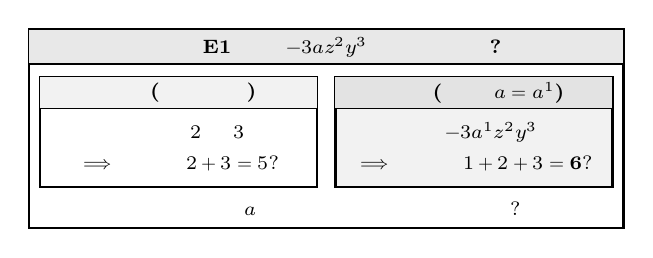
\begin{tikzpicture}[x=1cm, y=1cm, every node/.style={font=\scriptsize, text=black}]
  \draw[black, line width=0.9pt] (0,0) rectangle (7.55,2.52);
  \fill[gray!18] (0,2.08) rectangle (7.55,2.52);
  \draw[black, line width=0.6pt] (0,2.08) -- (7.55,2.08);
  \node at (3.775,2.30) {\textbf{បេសកកម្ម \en{E1}៖ តើឯកធា $-3az^2y^3$ មានដឺក្រេស្មើប៉ុន្មាន?}};

  % Left: Student A (Forgets hidden exponent 1)
  \draw[black, line width=0.8pt] (0.14,0.52) rectangle (3.66,1.92);
  \fill[gray!10] (0.14,1.52) rectangle (3.66,1.92);
  \draw[black, line width=0.5pt] (0.14,1.52) -- (3.66,1.52);
  \node at (1.90,1.72) {\textbf{សិស្ស ក (មើលតែលេខស្វ័យគុណ)}};
  \node at (1.90,1.22) {ឃើញតែស្វ័យគុណ $2$ និង $3$};
  \node at (1.90,0.82) {$\implies$ ដឺក្រេស្មើ $2 + 3 = 5$?};

  % Right: Student B (Counts hidden exponent a^1)
  \draw[black, line width=0.95pt, fill=gray!10] (3.89,0.52) rectangle (7.41,1.92);
  \fill[gray!22] (3.89,1.52) rectangle (7.41,1.92);
  \draw[black, line width=0.55pt] (3.89,1.52) -- (7.41,1.52);
  \node at (5.65,1.72) {\textbf{សិស្ស ខ (រាប់ទាំង $a = a^1$)}};
  \node at (5.65,1.22) {សរសេរ $-3a^1z^2y^3$};
  \node at (5.65,0.82) {$\implies$ ដឺក្រេស្មើ $1 + 2 + 3 = \mathbf{6}$?};

  \node at (3.775,0.24) {\textbf{សំណួរគន្លឹះ៖} តើអថេរ $a$ ដែលគ្មានសរសេរលេខស្វ័យគុណ មាននិទស្សន្តប៉ុន្មាន?};
\end{tikzpicture}}

% ២. E2 Explore: គូបទ្រនុង 2a (ទំ.៥១) -> 2a, 4a^2, 8a^3 និងរចនាសម្ព័ន្ធឯកធា
\newcommand{\figCubeMonomialALGFiveOne}{%
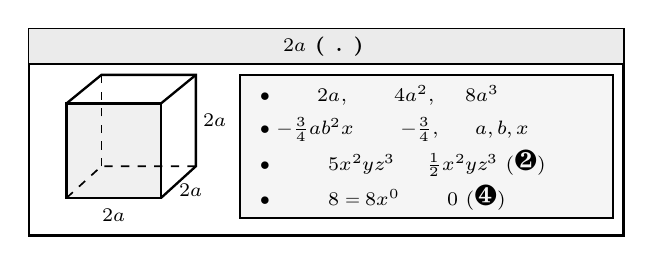
\begin{tikzpicture}[x=1cm, y=1cm, every node/.style={font=\scriptsize, text=black}]
  \draw[black, line width=0.9pt] (0,0) rectangle (7.55,2.62);
  \fill[gray!16] (0,2.18) rectangle (7.55,2.62);
  \draw[black, line width=0.6pt] (0,2.18) -- (7.55,2.18);
  \node at (3.775,2.40) {\textbf{ឧទាហរណ៍គូបទ្រនុង $2a$ (ទំ.៥១) និងធាតុផ្សំនៃឯកធា}};

  % Cube on left
  \draw[black, line width=0.9pt, fill=gray!12] (0.48,0.48) rectangle (1.68,1.68);
  \draw[black, line width=0.85pt] (1.68,0.48) -- (2.12,0.88) -- (2.12,2.04) -- (0.92,2.04) -- (0.48,1.68);
  \draw[black, line width=0.85pt] (1.68,1.68) -- (2.12,2.04);
  \draw[black, dashed, line width=0.6pt] (0.48,0.48) -- (0.92,0.88) -- (2.12,0.88);
  \draw[black, dashed, line width=0.6pt] (0.92,0.88) -- (0.92,2.04);
  \node at (1.08,0.26) {$2a$};
  \node at (2.06,0.58) {$2a$};
  \node at (2.36,1.46) {$2a$};

  % Monomial breakdown on right
  \draw[black, line width=0.8pt, fill=gray!8] (2.68,0.22) rectangle (7.42,2.04);
  \node[anchor=west] at (2.82,1.78) {$\bullet$ ទ្រនុង $2a$, មុខគូប $4a^2$, មាឌ $8a^3$};
  \node[anchor=west] at (2.82,1.35) {$\bullet$ $-\tfrac{3}{4}ab^2x$៖ មេគុណ $-\tfrac{3}{4}$, អថេរ $a,b,x$};
  \node[anchor=west] at (2.82,0.92) {$\bullet$ ដូចគ្នា៖ $5x^2yz^3$ និង $\tfrac{1}{2}x^2yz^3$ (\cnum{2})};
  \node[anchor=west] at (2.82,0.48) {$\bullet$ ចំនួនថេរ $8 = 8x^0$ ដឺក្រេ $0$ (\cnum{4})};
\end{tikzpicture}}

% ៣. E3 Explain: ផែនទីសម្គាល់ឯកធា ឯកធាដូចគ្នា និងដឺក្រេនៃឯកធា
\newcommand{\figRuleMapALGFiveOne}{%
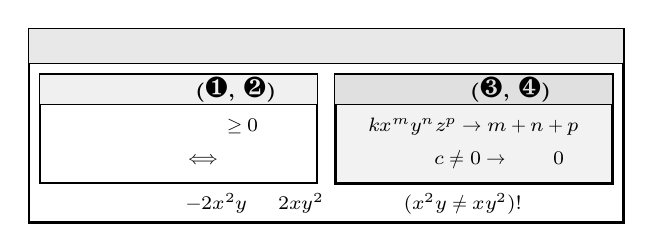
\begin{tikzpicture}[x=1cm, y=1cm, every node/.style={font=\scriptsize, text=black}]
  \draw[black, line width=0.9pt] (0,0) rectangle (7.55,2.46);
  \fill[gray!18] (0,2.02) rectangle (7.55,2.46);
  \draw[black, line width=0.6pt] (0,2.02) -- (7.55,2.02);
  \node at (3.775,2.24) {\textbf{សង្ខេបរចនាសម្ព័ន្ធឯកធា ឯកធាដូចគ្នា និងដឺក្រេនៃឯកធា}};

  % Left box: Monomial & Like Monomials
  \draw[black, line width=0.8pt] (0.14,0.50) rectangle (3.66,1.88);
  \fill[gray!12] (0.14,1.50) rectangle (3.66,1.88);
  \draw[black, line width=0.55pt] (0.14,1.50) -- (3.66,1.50);
  \node at (1.90,1.69) {\textbf{ឯកធា និងឯកធាដូចគ្នា (\cnum{1}, \cnum{2})}};
  \node at (1.90,1.22) {វិធីគុណ និងស្វ័យគុណគត់ $\ge 0$};
  \node at (1.90,0.80) {ផ្នែកអថេរដូចគ្នា $\iff$ ដូចគ្នា};

  % Right box: Degree of Monomial
  \draw[black, line width=0.95pt, fill=gray!10] (3.89,0.50) rectangle (7.41,1.88);
  \fill[gray!24] (3.89,1.50) rectangle (7.41,1.88);
  \draw[black, line width=0.6pt] (3.89,1.50) -- (7.41,1.50);
  \node at (5.65,1.69) {\textbf{ដឺក្រេនៃឯកធា (\cnum{3}, \cnum{4})}};
  \node at (5.65,1.22) {$kx^m y^n z^p \to m+n+p$};
  \node at (5.65,0.80) {ចំនួនថេរ $c \neq 0 \to$ ដឺក្រេ $0$};

  \node at (3.775,0.24) {\textbf{ប្រយ័ត្ន៖} $-2x^2y$ និង $2xy^2$ មិនដូចគ្នាទេ ($x^2y \neq xy^2$)!};
\end{tikzpicture}}

% ៤. E4 Elaborate: តារាងវិភាគឯកធា និងផ្គូផ្គងឯកធាដូចគ្នា (ទំ.៥២--៥៣)
\newcommand{\figElaborateALGFiveOne}{%
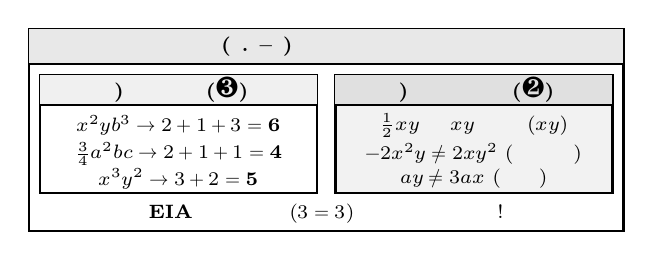
\begin{tikzpicture}[x=1cm, y=1cm, every node/.style={font=\scriptsize, text=black}]
  \draw[black, line width=0.9pt] (0,0) rectangle (7.55,2.56);
  \fill[gray!18] (0,2.12) rectangle (7.55,2.56);
  \draw[black, line width=0.6pt] (0,2.12) -- (7.55,2.12);
  \node at (3.775,2.34) {\textbf{លំហាត់គំរូ (ទំ.៥២--៥៣)៖ វិភាគដឺក្រេ និងជ្រើសរើសឯកធាដូចគ្នា}};

  \draw[black, line width=0.8pt] (0.14,0.48) rectangle (3.66,1.98);
  \fill[gray!12] (0.14,1.60) rectangle (3.66,1.98);
  \draw[black, line width=0.55pt] (0.14,1.60) -- (3.66,1.60);
  \node at (1.90,1.79) {\textbf{១) ដឺក្រេនៃឯកធា (\cnum{3})}};
  \node at (1.90,1.34) {$x^2yb^3 \to 2+1+3 = \mathbf{6}$};
  \node at (1.90,0.98) {$\tfrac{3}{4}a^2bc \to 2+1+1 = \mathbf{4}$};
  \node at (1.90,0.66) {$x^3y^2 \to 3+2 = \mathbf{5}$};

  \draw[black, line width=0.95pt, fill=gray!10] (3.89,0.48) rectangle (7.41,1.98);
  \fill[gray!24] (3.89,1.60) rectangle (7.41,1.98);
  \draw[black, line width=0.6pt] (3.89,1.60) -- (7.41,1.60);
  \node at (5.65,1.79) {\textbf{២) ជ្រើសឯកធាដូចគ្នា (\cnum{2})}};
  \node at (5.65,1.34) {$\tfrac{1}{2}xy$ និង $xy$ ដូចគ្នា ($xy$)};
  \node at (5.65,0.98) {$-2x^2y \neq 2xy^2$ (ខុសស្វ័យគុណ)};
  \node at (5.65,0.66) {$ay \neq 3ax$ (ខុសអថេរ)};

  \node at (3.775,0.22) {\textbf{\en{EIA}៖} ដឺក្រេស្មើគ្នា ($3=3$) មិនធានាថាជាឯកធាដូចគ្នាឡើយ!};
\end{tikzpicture}}

% ៥. E5 Evaluate: ជម្រើសវិនិច្ឆ័យ A-D (ជ្រើសឯកធាដូចគ្នានឹង -5a^2b^3)
\newcommand{\figExitALGFiveOne}{%
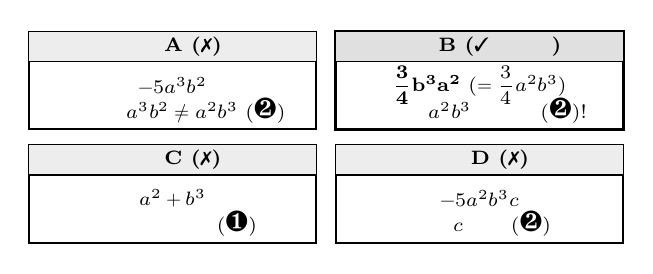
\begin{tikzpicture}[x=1cm, y=1cm, every node/.style={font=\scriptsize, text=black}]
  % Choice A
  \draw[black, line width=0.8pt] (0,1.44) rectangle (3.65,2.68);
  \fill[gray!14] (0,2.30) rectangle (3.65,2.68);
  \draw[black, line width=0.5pt] (0,2.30) -- (3.65,2.30);
  \node at (1.825,2.49) {\textbf{ជម្រើស \en{A} (\ding{55})}};
  \node at (1.825,2.00) {$-5a^3b^2$};
  \node at (1.825,1.68) {ខុសស្វ័យគុណ $a^3b^2 \neq a^2b^3$ (\cnum{2})};

  % Choice B (Correct)
  \draw[black, line width=1.05pt] (3.90,1.44) rectangle (7.55,2.68);
  \fill[gray!24] (3.90,2.30) rectangle (7.55,2.68);
  \draw[black, line width=0.6pt] (3.90,2.30) -- (7.55,2.30);
  \node at (5.725,2.49) {\textbf{ជម្រើស \en{B} (\ding{51} ត្រឹមត្រូវ)}};
  \node at (5.725,2.00) {$\mathbf{\dfrac{3}{4}b^3a^2}$ ($= \dfrac{3}{4}a^2b^3$)};
  \node at (5.725,1.68) {ផ្នែកអថេរ $a^2b^3$ ដូចគ្នាគត់ (\cnum{2})!};

  % Choice C
  \draw[black, line width=0.8pt] (0,0) rectangle (3.65,1.24);
  \fill[gray!14] (0,0.86) rectangle (3.65,1.24);
  \draw[black, line width=0.5pt] (0,0.86) -- (3.65,0.86);
  \node at (1.825,1.05) {\textbf{ជម្រើស \en{C} (\ding{55})}};
  \node at (1.825,0.56) {$a^2 + b^3$};
  \node at (1.825,0.24) {មានសញ្ញាបូក មិនមែនឯកធា (\cnum{1})};

  % Choice D
  \draw[black, line width=0.8pt] (3.90,0) rectangle (7.55,1.24);
  \fill[gray!14] (3.90,0.86) rectangle (7.55,1.24);
  \draw[black, line width=0.5pt] (3.90,0.86) -- (7.55,0.86);
  \node at (5.725,1.05) {\textbf{ជម្រើស \en{D} (\ding{55})}};
  \node at (5.725,0.56) {$-5a^2b^3c$};
  \node at (5.725,0.24) {លើសអថេរ $c$ មួយទៀត (\cnum{2})};
\end{tikzpicture}}

\begin{document}
\fontsize{10pt}{15.2pt}\selectfont

% ============================================================================
% ក្បាលរដ្ឋបាល (Administrative Header — តាមគំរូ ls_plan.tex)
% ============================================================================
{\centering
  {\muol\fontsize{11pt}{16pt}\selectfont ព្រះរាជាណាចក្រកម្ពុជា\par}
  {\muol\fontsize{11pt}{16pt}\selectfont ជាតិ សាសនា ព្រះមហាក្សត្រ\par}
  \vspace{-3pt}{\khmflourish\par}
}

\vspace{1pt}
{\muol\fontsize{10pt}{15.5pt}\selectfont
មន្ទីរអប់រំ យុវជន និងកីឡា ខេត្តកំពង់ធំ\par
ការិយាល័យអប់រំ យុវជន និងកីឡា ស្រុកកំពង់ស្វាយ\par
អនុវិទ្យាល័យព្រះក្រសាំង\par}

\vspace{2pt}
{\centering{\muol\fontsize{11.5pt}{17pt}\selectfont កិច្ចតែងការបង្រៀន\par}}
\vspace{2pt}

% --- ព័ត៌មានទូទៅ ---
{\hspace*{2.8cm}\renewcommand{\arraystretch}{1.08}
\begin{tabular}{@{}l@{\hspace{0.35cm}}p{2.9cm}@{\hspace{0.15cm}}c@{\hspace{0.25cm}}l@{}}
  - & មុខវិជ្ជា & : & គណិតវិទ្យា ថ្នាក់ទី៨ (ពីជគណិត) \\
  - & ចំណងជើងមេរៀន & : & មេរៀនទី៥៖ កន្សោមពីជគណិត \\
  - & ចំណងជើងរង & : & ១.១ សញ្ញាណឯកធា, ១.២ ឯកធាដូចគ្នា និង ១.៣ ដឺក្រេនៃឯកធា \\
  - & រយៈពេល & : & ១ ម៉ោងសិក្សា (៥០ នាទី) \\
  - & បង្រៀនដោយ & : & ហុក ប៊ុនថែន \\
  - & កាលបរិច្ឆេទ & : & ថ្ងៃសុក្រ ទី៤ ខែធ្នូ ឆ្នាំ២០២៦ \\
\end{tabular}\par}

\vspace{2pt}

% --- I. វត្ថុបំណង ---
{\muol\fontsize{10pt}{15.5pt}\selectfont \enbf{I.} វត្ថុបំណង\par}
\vspace{1pt}
{\renewcommand{\arraystretch}{1.10}
\begin{tabular}{@{}p{0.55cm}@{}p{2.35cm}@{\hspace{0.15cm}}c@{\hspace{0.25cm}}p{14.95cm}@{}}
  \hfill\wcirc\hspace{0.2cm} & វិជ្ជាសម្បទា & : & សិស្សប្រាប់និយមន័យកន្សោមពីជគណិត ឯកធា (មេគុណនិងផ្នែកអថេរ) ឯកធាដូចគ្នា និងដឺក្រេនៃឯកធា (រួមទាំងចំនួនថេរដែលមានដឺក្រេសូន្យ) បានត្រឹមត្រូវ ។ \\
  \hfill\wcirc\hspace{0.2cm} & បំណិនសម្បទា & : & សិស្សញែកសម្គាល់ឯកធា កំណត់មេគុណនិងអថេរ ជ្រើសរើសគូឯកធាដូចគ្នា និងគណនាដឺក្រេនៃឯកធាលើសន្លឹកកិច្ចការ (ទំ.៥១--៥៣, ៧២) បានត្រឹមត្រូវ ។ \\
  \hfill\wcirc\hspace{0.2cm} & ចរិយាសម្បទា & : & សិស្សមានទម្លាប់ពិនិត្យសង្កេតនិទស្សន្តនិងអថេរយ៉ាងល្អិតល្អន់ ជៀសវាងការភាន់ច្រឡំផ្នែកអថេរក្នុងប្រមាណវិធីពិជគណិត ។ \\
\end{tabular}\par}

\vspace{2pt}

% --- II. សម្ភារៈឧបទេស ---
{\muol\fontsize{10pt}{15.5pt}\selectfont \enbf{II.} សម្ភារៈឧបទេស\par}
\vspace{1pt}
\hspace*{0.55cm}$\bullet$\ សៀវភៅសិក្សាគោលថ្នាក់ទី៨ (ទំ.៥១--៥៣, ៧២) ក្ដារខៀន ដីស/ហ្វឺត បន្ទាត់ត្រង់ និង\textbf{សន្លឹកកិច្ចការសិស្សបំពេញចន្លោះ ស-ខ្មៅ} (កូដ \en{ALG51} ទំព័រ ១--២ សម្រាប់សិស្ស និងទំព័រ ៣ ប្លង់ក្ដារខៀន/ចម្លើយគ្រូ — គ្មានប្រើ \en{LCD})\par

\vspace{2pt}

% --- III. វិធីសាស្រ្តបង្រៀន ---
{\muol\fontsize{10pt}{15.5pt}\selectfont \enbf{III.} វិធីសាស្រ្តបង្រៀន\par}
\vspace{1pt}
{\renewcommand{\arraystretch}{1.08}
\begin{tabular}{@{}p{0.55cm}@{}p{2.35cm}@{\hspace{0.15cm}}c@{\hspace{0.25cm}}p{14.95cm}@{}}
  \hfill$\bullet$\hspace{0.2cm} & គោលវិធី & : & សិស្សមជ្ឈមណ្ឌល (សន្លឹកកិច្ចការបំពេញចន្លោះជាគោល + ការពិភាក្សាជាក្រុមតូច ៣ នាក់) \\
  \hfill$\bullet$\hspace{0.2cm} & យុទ្ធវិធីបង្រៀន & : & គំរូស្ថាបនានិយម \en{5Es} រួមបញ្ចូល \textbf{គំរូធរណីមាត្រគូបទ្រនុង $2a$} និង \textbf{តារាងញែកមេគុណ--ផ្នែកអថេរ--និទស្សន្តលាក់មុខ $1$} \\
\end{tabular}\par}

\vspace{2pt}

% --- IV. ដំណើរការបង្រៀន ---
{\muol\fontsize{10pt}{15.5pt}\selectfont \enbf{IV.} ដំណើរការបង្រៀន\par}

{\renewcommand{\arraystretch}{1.15}
\begin{longtable}{|L{5.50cm}|L{7.90cm}|L{4.80cm}|}
\hline
\multicolumn{1}{|c|}{\cellcolor{headgray}\muol សកម្មភាពគ្រូ} &
\multicolumn{1}{c|}{\cellcolor{headgray}\muol ខ្លឹមសារមេរៀន} &
\multicolumn{1}{c|}{\cellcolor{headgray}\muol សកម្មភាពសិស្ស} \\
\hline
\endfirsthead

\hline
\multicolumn{1}{|c|}{\cellcolor{headgray}\muol សកម្មភាពគ្រូ} &
\multicolumn{1}{c|}{\cellcolor{headgray}\muol ខ្លឹមសារមេរៀន} &
\multicolumn{1}{c|}{\cellcolor{headgray}\muol សកម្មភាពសិស្ស} \\
\hline
\endhead

% ==================== ជំហានទី១ (2min) ====================
\stepheader{ជំហានទី១ \enbf{(}រដ្ឋបាលថ្នាក់\enbf{)}}
$\bullet$ ពិនិត្យវត្តមាន អនាម័យ និងសណ្ដាប់ធ្នាប់ថ្នាក់រៀន \par
$\bullet$ រៀបចំក្រុមតូច ៣ នាក់តាមតុ និងចែក\textbf{សន្លឹកកិច្ចការសិស្ស (\en{ALG51} ទំព័រ ១–២)}
&
$\bullet$ រដ្ឋបាលថ្នាក់ អនាម័យ និងវិន័យសិក្សា \par
$\bullet$ ចែកសន្លឹកកិច្ចការម្នាក់ ១ សន្លឹក សម្រាប់បំពេញតាមដំណាក់កាល \en{E1--E5}
&
$\circ$ ប្រធានថ្នាក់រាយការណ៍វត្តមានសិស្ស \par
$\circ$ ទទួលសន្លឹកកិច្ចការ សរសេរឈ្មោះ និងអង្គុយតាមក្រុម ៣ នាក់ \\
\hline

% ==================== ជំហានទី២ (9min: កំណែ <=3m + រំលឹក 3m + E1 3m) ====================
\stepheader{ជំហានទី២ \enbf{(}កិច្ចការផ្ទះ \enbf{+} ទំនាក់ទំនងមេរៀនថ្មី\enbf{)}}
\ditem \textbf{កំណែកិច្ចការផ្ទះ ($\le\text{\enbf{3\,min}}$)} \par
$\bullet$ ហៅសិស្ស ២ នាក់ឡើងកែលំហាត់ទំ.៥០ លេខ ៨ និង លេខ ៩ លើក្ដារខៀន
&
{\centering\redsub{កំណែកិច្ចការផ្ទះមេរៀនមុន (ទំ.៥០ \#8 និង \#9)}\par}
$\bullet$ \textbf{\#8 (រតនាដើរ $0.8\unit{km}$ ល្បឿន $5\unit{km/h}$)៖} $t = 9\unit{mn}\,36\unit{s} \implies$ ចេញម៉ោង $\mathbf{6\unit{h}\,35\unit{mn}\,24\unit{s}}$ \par
$\bullet$ \textbf{\#9 (សុខានិងមករា $291\unit{km}, 60+40=100\unit{km/h}$)៖} $t = 2.91\unit{h} \implies$ ជួបម៉ោង $\mathbf{9\unit{h}\,54\unit{mn}\,36\unit{s}}$
&
$\circ$ ផ្ទៀងចម្លើយ និងកែតម្រូវចូលសៀវភៅកិច្ចការផ្ទះ \\[3pt]

\ditem \textbf{រំលឹកមេរៀនទាក់ទង (\enbf{3min})} \par
$\bullet$ សួរ៖ «បើគូបមួយមានទ្រនុងប្រវែង $a$ តើផ្ទៃមុខមួយ និងមាឌរបស់វាស្មើអ្វី?»
&
{\centering\redsub{រំលឹកផ្ទៃក្រឡា មាឌគូប និងស្វ័យគុណសូន្យ}\par}
$\bullet$ គូបទ្រនុង $a$៖ ផ្ទៃមុខមួយ $S = a^2$, មាឌគូប $V = a^3$
&
$\circ$ ឆ្លើយ៖ «ផ្ទៃមុខមួយស្មើ $a^2$ និងមាឌគូបស្មើ $a^3$!» \\[3pt]

$\bullet$ សួរបន្ត៖ «ចុះចំពោះ $x\neq 0$ តើ $x^0$ ស្មើប៉ុន្មាន? ចុះអក្សរ $a$ ស្មើ $a$ ស្វ័យគុណប៉ុន្មាន?»
&
$\bullet$ ស្វ័យគុណ៖ $x^0 = 1\ (x\neq 0)$ និង $a = a^1$
&
$\circ$ ឆ្លើយ៖ «$x^0 = 1$ ហើយ $a = a^1$!» \\[3pt]

\fiveE{E1 - Engage (3min)} \timenote{(កុំទាន់ផ្ដល់ចម្លើយ)} \par
\ditem \textbf{បេសកកម្មអន្ទាក់ដឺក្រេនៃឯកធា (សន្លឹកកិច្ចការ \en{E1})} \par
$\bullet$ ឱ្យសិស្សអានប្រអប់ \en{E1} ហើយគូសជ្រើសរើសរវាង\textbf{សិស្ស ក} និង\textbf{សិស្ស ខ}
&
\redsub{បេសកកម្ម \en{E1}៖ តើកន្សោម $-3az^2y^3$ មានដឺក្រេស្មើប៉ុន្មាន?} \par
$\bullet$ \textbf{សិស្ស ក} ឃើញតែលេខស្វ័យគុណ $2$ និង $3$ ក៏ថាដឺក្រេស្មើ $2 + 3 = 5$! \par
$\bullet$ \textbf{សិស្ស ខ} រាប់ទាំងនិទស្សន្ត $1$ លើអថេរ $a$ ($a = a^1$) ថាដឺក្រេស្មើ $1 + 2 + 3 = 6$! តើអ្នកណាត្រូវ?
&
$\circ$ ពិភាក្សាជាគូ និងគូស \ding{51} ក្នុងប្រអប់ \en{E1} លើសន្លឹកកិច្ចការ \\[3pt]

&
\cfig{\figEngageALGFiveOne}
& \\
\hline

% ==================== ជំហានទី៣ (17min: E2 11m + E3 6m) ====================
\stepheader{ជំហានទី៣ \enbf{(}ខ្លឹមសារមេរៀនថ្មី\enbf{)}}
\fiveE{E2 - Explore (11min)} \par
$\bullet$ សរសេរចំណងជើងមេរៀនទី៥ និងចំណងជើងរង \textbf{១. ឯកធា} លើក្ដារខៀន \par
\ditem \textbf{សកម្មភាព ១៖ សញ្ញាណឯកធា មេគុណ និងអថេរ (ទំ.៥១–៥២, \enbf{6min}, \en{E2-A})} \par
$\bullet$ ឱ្យសិស្សបំពេញផ្ទៃមុខនិងមាឌគូបទ្រនុង $2a$ រួចញែកមេគុណនិងអថេរលើ \en{E2-A}
&
មេរៀនទី៥ \quad {\muol កន្សោមពីជគណិត} \par
១. ឯកធា \quad (១.១ សញ្ញាណឯកធា, ១.២ ឯកធាដូចគ្នា, ១.៣ ដឺក្រេនៃឯកធា) \par
$\bullet$ \textbf{គូបទ្រនុង $2a$ (ទំ.៥១)៖} ផ្ទៃមុខខាងនីមួយៗ $(2a)^2 = 4a^2$; មាឌគូប $(2a)^3 = 8a^3$ \par
$\bullet$ រង្វាស់ $2a, 4a^2, 8a^3$ តាងដោយចំនួននិងអថេរ ហៅថា \textbf{កន្សោមពីជគណិត} ។ កន្សោមដែលមានតែប្រមាណវិធីគុណនិងស្វ័យគុណនិទស្សន្តគត់វិជ្ជមានឬសូន្យ ហៅថា \textbf{ឯកធា} ($7x^2y, -\tfrac{3}{4}a^2b^4, \sqrt{3}x^2yt, 8 = 8x^0$)
&
$\circ$ គណនាឃើញ $4a^2, 8a^3$ និងសង្កេតលក្ខណៈសម្គាល់ឯកធា \\[3pt]

$\bullet$ ឱ្យសិស្សបំពេញលំហាត់គំរូ និងប្រតិបត្តិទី ១–២ (ទំ.៥២) លើសន្លឹកកិច្ចការ \en{E2-A}
&
$\bullet$ \textbf{មេគុណ និងអថេរ (ទំ.៥១–៥២)៖} ចំពោះ $7x^2y$ មាន $7$ ជា\textbf{មេគុណ} និង $x, y$ ជា\textbf{អថេរ}; ឯ $-\tfrac{3}{4}ab^2x$ មានមេគុណ $-\tfrac{3}{4}$ និងអថេរ $a, b, x$ \par
$\bullet$ \textbf{ញែកឯកធា (ប្រតិបត្តិទី ២ ទំ.៥២)៖} $\tfrac{1}{5}x^2y$ និង $zx^2a^3b^4$ ជាឯកធា; ឯ $3x^2 + 2$ និង $25 - \tfrac{2}{3}a^4bc^2$ មិនមែនជាឯកធាទេ (មានសញ្ញាបូក/ដកភ្ជាប់តួ)
&
$\circ$ បញ្ជាក់មេគុណ អថេរ និងញែកឯកធាបានត្រឹមត្រូវ \\[3pt]

&
\cfig{\figCubeMonomialALGFiveOne}
& \\[3pt]

\ditem \textbf{សកម្មភាព ២៖ ឯកធាដូចគ្នា និងដឺក្រេនៃឯកធា (ទំ.៥២–៥៣, \enbf{5min}, \en{E2-B})} \par
$\bullet$ ឱ្យសិស្សប្រៀបធៀបផ្នែកអថេរនៃ $-3xbc^2$ និង $\tfrac{2}{3}xbc^2$ រួចគណនាដឺក្រេនៃ $3x, 2xy, ax^2y$
&
$\bullet$ \textbf{១.២ ឯកធាដូចគ្នា (ទំ.៥២)៖} $-3xbc^2$ និង $\tfrac{2}{3}xbc^2$ មានផ្នែកអថេរ $xbc^2$ ដូចគ្នា ហៅថា \textbf{ឯកធាដូចគ្នា} (ដូចគ្នាដែរ៖ $5x^2yz^3$ និង $\tfrac{1}{2}x^2yz^3$) \par
$\bullet$ \textbf{១.៣ ដឺក្រេនៃឯកធា (ទំ.៥២)៖} $3x$ (ដឺក្រេ $1$), $2xy$ ($1+1=2$), $ax^2y$ ($1+2+1=4$)
&
$\circ$ រកឃើញថាដឺក្រេនៃឯកធាស្មើផលបូកនិទស្សន្តនៃអថេរទាំងអស់ \\[3pt]

% --- E3 Explain (6min) ---
\fiveE{E3 - Explain (6min)} \par
$\bullet$ ដឹកនាំសិស្សសង្ខេបនិយមន័យ\textbf{ឯកធា ឯកធាដូចគ្នា និងដឺក្រេនៃឯកធា} (ទំ.៥១–៥២)
&
$\bullet$ \textbf{និយមន័យគោល (ទំ.៥១–៥២)៖} \par
\hspace*{0.15cm}១) \textbf{ឯកធា៖} កន្សោមពីជគណិតដែលមានតែប្រមាណវិធីគុណ និងស្វ័យគុណនិទស្សន្តគត់វិជ្ជមានឬសូន្យ \par
\hspace*{0.15cm}២) \textbf{ឯកធាដូចគ្នា៖} ឯកធាដែលមាន\graybox{ផ្នែកអថេរដូចគ្នា} \quad ៣) \textbf{ដឺក្រេឯកធា៖} \graybox{ផលបូកនិទស្សន្តនៃអថេរទាំងអស់}
&
$\circ$ បំពេញប្រអប់និយមន័យលើសន្លឹកកិច្ចការ \en{E3} \\[3pt]

&
\cfig{\figRuleMapALGFiveOne}
& \\[3pt]

$\bullet$ ភ្ជាប់\textbf{ធនាគារហេតុផល \cnum{1}--\cnum{4}} លើក្ដារខៀន និងសន្លឹកកិច្ចការ
&
\textbf{ធនាគារហេតុផល (\en{Warrant Bank})៖} \par
\cnum{1} \textbf{លក្ខខណ្ឌឯកធា៖} គ្មានសញ្ញាបូក/ដកភ្ជាប់តួ គ្មានអថេរនៅភាគបែង ឬក្នុងរ៉ាឌីកាល់ \par
\cnum{2} \textbf{ឯកធាដូចគ្នា៖} ផ្នែកអថេរដូចគ្នាទាំងអក្សរ ទាំងនិទស្សន្តតាមអក្សរនីមួយៗ ($b^3a^2 = a^2b^3$) \par
\cnum{3} \textbf{និទស្សន្តលាក់មុខ $1$៖} អថេរគ្មានសរសេរស្វ័យគុណមាននិទស្សន្ត $1$ ($a = a^1$) \par
\cnum{4} \textbf{ដឺក្រេចំនួនថេរ៖} ចំនួនថេរ $c \neq 0$ អាចសរសេរ $cx^0$ ដូច្នេះមានដឺក្រេស្មើ $0$
&
$\circ$ ផ្ទៀងលេខកូដ \cnum{1}--\cnum{4} លើសន្លឹកកិច្ចការ \\
\hline

% ==================== ជំហានទី៤ (20min: E4 10m + E5 10m) ====================
\stepheader{ជំហានទី៤ \enbf{(}ពង្រីកចំណេះដឹង\enbf{)}}
\fiveE{E4 - Elaborate (10min)} \par
\ditem \textbf{លំហាត់គំរូ៖ តារាងដឺក្រេឯកធា និងការជ្រើសរើសឯកធាដូចគ្នា (ទំ.៥២–៥៣)} \par
$\bullet$ ឱ្យសិស្សបំពេញតារាងអថេរនិងដឺក្រេ ព្រមទាំងជ្រើសគូឯកធាដូចគ្នាលើសន្លឹកកិច្ចការ \en{E4}
&
{\muol លំហាត់គំរូ} \textbf{(ទំ.៥២–៥៣)៖} \par
$\bullet$ \textbf{១) កំណត់អថេរ និងដឺក្រេនៃឯកធា (\cnum{3})៖} \par
\hspace*{0.2cm}-- $x^2yb^3$៖ អថេរ $x, y, b$ ដឺក្រេ $2+1+3 = \graybox{$6$}$; \quad $\tfrac{3}{4}a^2bc$៖ អថេរ $a, b, c$ ដឺក្រេ $2+1+1 = \graybox{$4$}$ \par
\hspace*{0.2cm}-- $x^3y^2$៖ អថេរ $x, y$ ដឺក្រេ $3+2 = \graybox{$5$}$; \quad $-3az^2y^3$៖ អថេរ $a, z, y$ ដឺក្រេ $1+2+3 = \graybox{$6$}$ \par
$\bullet$ \textbf{២) ជ្រើសឯកធាដូចគ្នា (ប្រតិបត្តិទំ.៥២៖ $\tfrac{1}{2}xy, -2x^2y, ay, 3ax, 2xy^2, xy$)៖} \par
\hspace*{0.2cm}មានតែ \graybox{$\tfrac{1}{2}xy$ និង $xy$} ប៉ុណ្ណោះដែលជាឯកធាដូចគ្នា (\cnum{2})!
&
$\circ$ បំពេញតារាងដឺក្រេ ($6, 4, 5, 6$) និងជ្រើសបានគូ $\tfrac{1}{2}xy, xy$ \\[3pt]

&
\cfig{\figElaborateALGFiveOne}
& \\[3pt]

$\bullet$ សួរសំណួរឆ្លុះបញ្ចាំង \textbf{\en{EIA Looking-Back} (1min)}
&
\textbf{\en{EIA Looking-Back}៖} «ហេតុអ្វី $-2x^2y$ និង $2xy^2$ មិនមែនជាឯកធាដូចគ្នា ទោះបីមានអក្សរ $x, y$ និងដឺក្រេ $3$ ស្មើគ្នាក៏ដោយ?» ($\to$ ព្រោះស្វ័យគុណលើ $x$ និង $y$ ខុសគ្នា៖ $x^2y \neq xy^2$!)
&
$\circ$ ពន្យល់ថាត្រូវដូចគ្នាទាំងនិទស្សន្តលើអថេរនីមួយៗ \\[3pt]

% --- E5 Evaluate (10min) ---
\fiveE{E5 - Evaluate (10min)} \par
\ditem \textbf{ប្រតិបត្តិជាក្រុមតូច ៣ នាក់ (4min, សន្លឹកកិច្ចការ \en{E5})} \par
$\bullet$ ឱ្យសិស្សដោះស្រាយប្រតិបត្តិទី ១ (ទំ.៥២) និងប្រតិបត្តិដឺក្រេ (ទំ.៥៣ ក, ខ, គ)
&
{\muol លំហាត់ប្រតិបត្តិ} \textbf{(ទំ.៥២–៥៣)៖} \par
$\bullet$ \textbf{១) ប្រតិបត្តិទី ១ (ទំ.៥២)៖} ឯកធា $2\sqrt{3}yt^2$ មានមេគុណ \graybox{$2\sqrt{3}$}, អថេរ $y, t$ និងដឺក្រេ $1+2 = \mathbf{3}$ \par
$\bullet$ \textbf{២) ប្រតិបត្តិទំ.៥៣៖} ក) $\tfrac{1}{2}xyz$ (ដឺក្រេ $\mathbf{3}$); \quad ខ) $8x^3yz^2$ (ដឺក្រេ $\mathbf{6}$); \quad គ) $14$ (គ្មានអថេរ ដឺក្រេ $\mathbf{0}$ តាម \cnum{4})
&
$\circ$ គណនាជាក្រុមឃើញមេគុណ $2\sqrt{3}$ និងដឺក្រេ $3, 6, 0$ \\[3pt]

$\bullet$ ឱ្យក្រុមសិស្សផ្ទៀងផ្ទាត់និង\textbf{បិទបេសកកម្ម \en{E1} (2min)}
&
$\bullet$ \textbf{បិទបេសកកម្ម \en{E1}៖} សិស្ស ខ ត្រឹមត្រូវ! $-3az^2y^3 = -3a^1z^2y^3$ មានដឺក្រេ $1 + 2 + 3 = \mathbf{6}$!
&
$\circ$ បិទបេសកកម្ម \en{E1} ឃើញសិស្ស ខ ត្រឹមត្រូវ (ដឺក្រេ $6$) \\[3pt]

\ditem \textbf{សំណួរវិនិច្ឆ័យ \en{A--D} និងសំបុត្រចេញ (4min)} \par
$\bullet$ ឱ្យសិស្សគូសរង្វង់ជម្រើសត្រូវលើសន្លឹកកិច្ចការ រួចលើកម្រាមដៃ ១--៤
&
{\centering\textbf{សំណួរវិនិច្ឆ័យ \en{A--D}៖ តើកន្សោមមួយណាជាឯកធាដូចគ្នានឹងឯកធា $-5a^2b^3$?}\par}
&
$\circ$ វិភាគជម្រើស \en{A--D} និងលើកម្រាមដៃ ២ (\textbf{ជម្រើស \en{B}}) \\[3pt]

&
\cfig{\figExitALGFiveOne}
& \\[3pt]

$\bullet$ បញ្ជាក់ចម្លើយត្រូវ (\textbf{ជម្រើស \en{B}}) និងឱ្យបំពេញ\textbf{សំបុត្រចេញ ៦០ វិនាទី}
&
$\bullet$ \textbf{សំបុត្រចេញ៖} ឯកធា $-7xy^4z$ មានមេគុណស្មើ $\mathbf{-7}$ និងមានដឺក្រេស្មើ $1+4+1 = \mathbf{6}$ ។
&
$\circ$ បំពេញសំបុត្រចេញលើសន្លឹកកិច្ចការមុនបញ្ចប់ម៉ោង \\
\hline

% ==================== ជំហានទី៥ (<=2min) ====================
\stepheader{ជំហានទី៥ \enbf{(}កិច្ចការផ្ទះ \enbf{+} បណ្ដាំផ្ញើ\enbf{)}}
\timenote{ចំណាយពេលឱ្យតិចបំផុតកុំឱ្យលើស 2min} \par
$\bullet$ ណែនាំប្រអប់\textbf{កិច្ចការផ្ទះ}លើសន្លឹកកិច្ចការទំព័រ ២ (ទំ.៥៣ ង, ច, ឆ និងទំ.៧២ លេខ ១)
&
{\centering{\muol កិច្ចការផ្ទះ} \textbf{(សៀវភៅគោល ទំ.៥៣ និង ទំ.៧២ លេខ ១)}\par} \par
$\bullet$ \textbf{១) ប្រតិបត្តិទំ.៥៣ (ង, ច, ឆ)៖} កំណត់អថេរនិងរកដឺក្រេនៃឯកធា៖ ង) $21ab^4c$, \ ច) $3x^2y^3z^4$, \ ឆ) $axyz$ ។ \par
$\bullet$ \textbf{២) លំហាត់ \#1 (ទំ.៧២)៖} តើកន្សោមណាខ្លះជាឯកធា៖ $\dfrac{x^3}{3}, \ \sqrt{5}ax^2, \ \dfrac{7xy^2}{3}, \ x+2y, \ \dfrac{a}{x^2}, \ x(x+y)$?
&
$\circ$ គូសចំណាំកិច្ចការផ្ទះទំ.៥៣ និងទំ.៧២ \#1 \\[3pt]

$\bullet$ ផ្ដាំផ្ញើឱ្យអានមុនចំណុច ១.៤–១.៦ (ប្រមាណវិធីបូក ដក គុណ និងចែកឯកធា)
&
$\bullet$ \textbf{បណ្ដាំផ្ញើ៖} អានមុន \textbf{១.៤–១.៦ ប្រមាណវិធីលើឯកធា (ទំ.៥៣–៥៦)} សម្រាប់ម៉ោងបន្ទាប់ ។
&
$\circ$ កត់ត្រាបណ្ដាំផ្ញើ ទុកសន្លឹកកិច្ចការក្នុងសៀវភៅ និងជម្រាបលាគ្រូ \\
\hline
\end{longtable}}

\vspace{6pt}
% --- ហត្ថលេខា (កាលបរិច្ឆេទត្រូវគ្នា ១០០% នឹងខាងលើ) ---
{\centering
\hspace*{5.2cm}\begin{minipage}{11.5cm}
  \centering
  ថ្ងៃសុក្រ ១០រោច ខែកត្តិក ឆ្នាំមមី អដ្ឋស័ក ពុទ្ធសករាជ ២៥៧០\par
  កំពង់ស្វាយ, ថ្ងៃទី៤ ខែធ្នូ ឆ្នាំ២០២៦\par
  \vspace{2pt}
  {\muol គ្រូបង្រៀន\par}
  \vspace{32pt}
  \hfill{\muol ហុក ប៊ុនថែន}\hspace*{1.4cm}
\end{minipage}\par}

\end{document}
